\chapter{Implementation and Results}

In this chapter, you will be acquainted with the implementation of the electric circuit consisting of BC547 NPN transistors, LEDs, Zener diodes, and resistors. Also a  clear description of performance analysis and the outcomes of the experiment are also provided.
\end{center}

%This is for reference only. Delete before finalization

\section{Implementation}

This project is being done by building a circuit on a bread board. The objective is to illustrate how transistors can be used as switches to control LED states in response to the changing voltage applications. The components of the project include:
\newline \textbf{1. Three BC547 NPN transistors:}
\newline The path for the current through the LEDs is established by these transistors which act as switches. Current limiting the base of each transistor is done by the resistor attached to it and connections will be made from a separate LED to each of the transistors.\cite{b10}
\newline \textbf{2. Three LEDs (red, yellow, and green):} 
\newline Each of the LEDs represents a different circuit state. A red LED represents the lowest voltage, a yellow LED represents the moderate voltage, and the green LED heralds the greatest voltage.\cite{b12}
\newline \textbf{3. Resistors:}
\newline The base resistors for the transistors are three 10kΩ resistors that are connected in order to limit the current passing through the Governor to the transistor’s base.
\newline Three 1kΩ resistors are used as current-limiting resistors in order to prevent LEDs from being damaged by overload currents.
\newline \textbf{4.Zener Diodes:}
\newline The 7.5V Zener Diode is utilized to maintain the specified voltage which prevents the circuit from receiving voltage beyond the designated level.
\newline The 10V and 12V Zener Diodes are then used in order to have LEDs show their different response to different voltage levels. Zener diodes are used to produce a constant voltage that can supply the required voltage to the transistor circuits.
\newline 12V Battery: A 12V source is used in order to power the entire circuit. It is able to provide enough voltage for both the LEDs and the transistors.\cite{10}
\newline \textbf{5.Male to Male Jumper Wires:}
\newline These wires carry the current flow without soldering the breadboard components.
\newline In this way, transistors are arranged in a switching configuration, and the Zener diodes control the voltage supplied to each transistor's base. The LEDs are accordingly lightened as the voltage goes up/down at the base of the transistor which is in turn managed by the Zener diodes.




\section{Performance Analysis}

The circuit's performance is analyzed by measuring the current through the LEDs and the transistor's switching behavior under different conditions. Important performance outputs are:
\newline \textbf{LED Brightness:} The brightness of each LED is a method to check the transistor's performance as a switch and also shows the Zener diodes' voltage stability.\cite{b13}
\newline \textbf{Current Limiting:} The current through the LEDs and transistors is measured to see if it is within safe limits.\cite{9}
\newline \textbf{Voltage Regulation:} The Zener diodes are tried to confirm if they can control the volts at certain levels (7.5 V, 10 V, and 12 V) and, hence, protect the circuit.\cite{8}
\newline Different voltage environments are applied during tests to investigate the action of each part as well as their responsibility for regulating current and LEDs.

\section{Results and Discussion}

\textbf{The experimental results showed that:}
The zener diodes were very good in holding the voltage at the expected values (7.5 V, 10 V, and 12 V), thus the circuit was stable and protected.
The BC547 transistors, by working as effective switches, enabled the current to pass through LEDs when the correct voltage was applied to the base.
The LEDs thus are perfectly matched to changes in voltage, with the red LED shining at the lower voltages, and the green LED only comes on at higher voltages, thus, current control leads to effective voltage control.
1k resistors with current limiting characteristics worked just fine in avoiding overcurrent that would damage the LED lights and help to prevent the longevity of these semiconductors through burning out.
The experimental results attest to the design concepts that involve transistors and Zener diodes in the LED-based system. Additionally, the design offers the possibility of optimization of different voltage levels and the use of additional LEDs or components.\cite{b16} Some pictures of the project in working state is given below-
\newline
The Red LED is glowing when 7.5 volt current is passing.It is shown in Figure: 3.1.
\begin{figure}[h!] % 'h' for placing it "here"
    \centering
    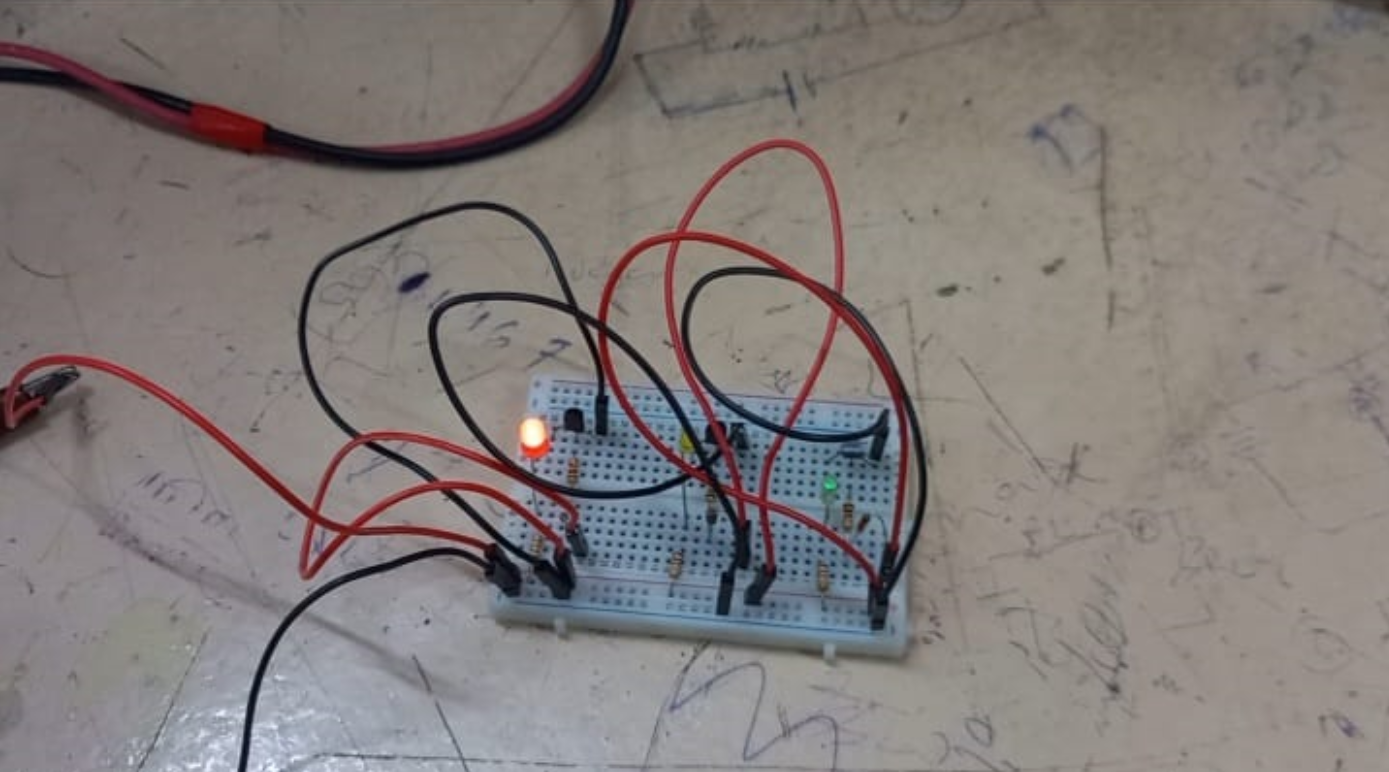
\includegraphics[width=0.5\textwidth]{10.png} % Replace 'diagram.png' with your image file
    \caption{Research Method}
    \label{fig:sample}
\end{figure}

\pagebreak
 The red and yellow LEDs are glowing when 10 volt is given.It is shown in Figure: 3.2.
\begin{figure}[h!] % 'h' for placing it "here"
    \centering
    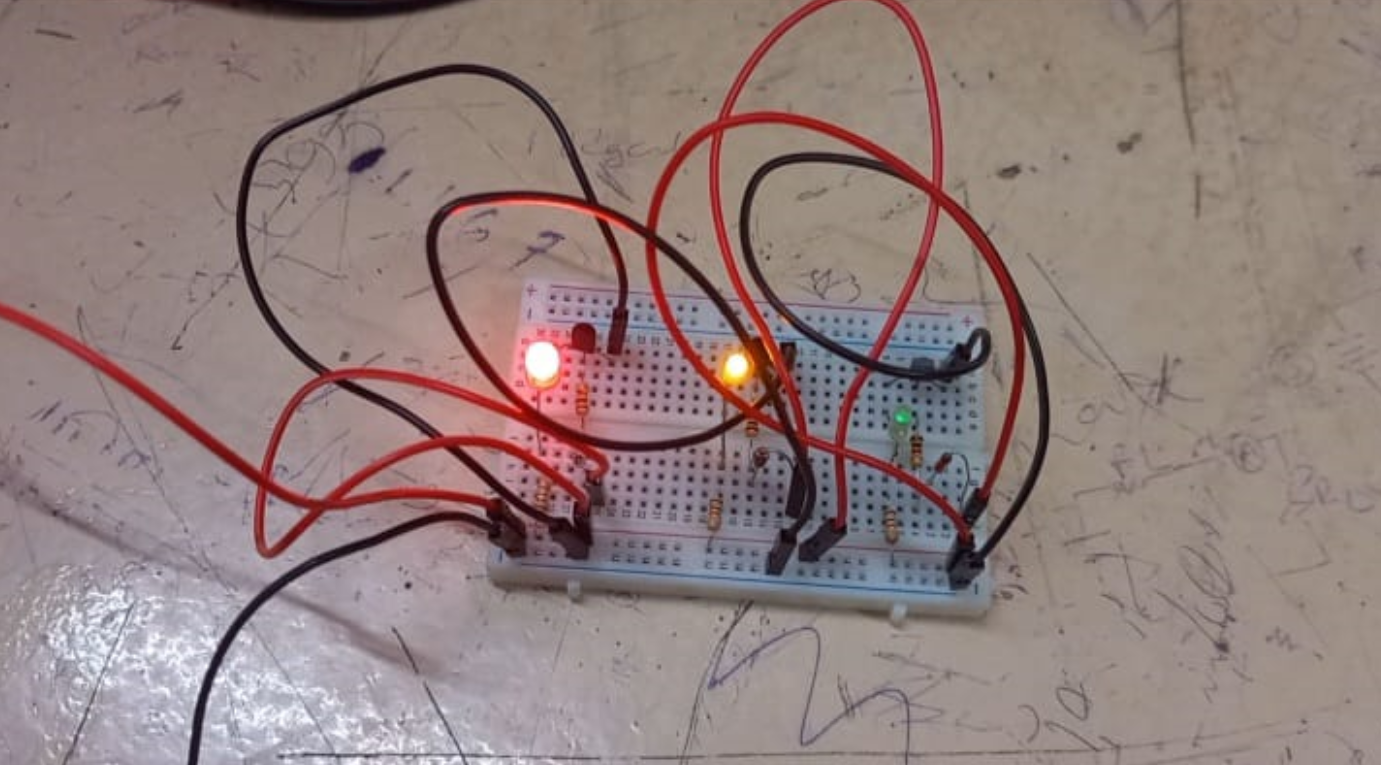
\includegraphics[width=0.5\textwidth]{11.png} % Replace 'diagram.png' with your image file
    \caption{Research Method}
    \label{fig:sample}
\end{figure}
\newline
All LEDs are glowing when 12 0r more volt is given.It is shown in Figure: 3.3.
\begin{figure}[h!] % 'h' for placing it "here"
    \centering
    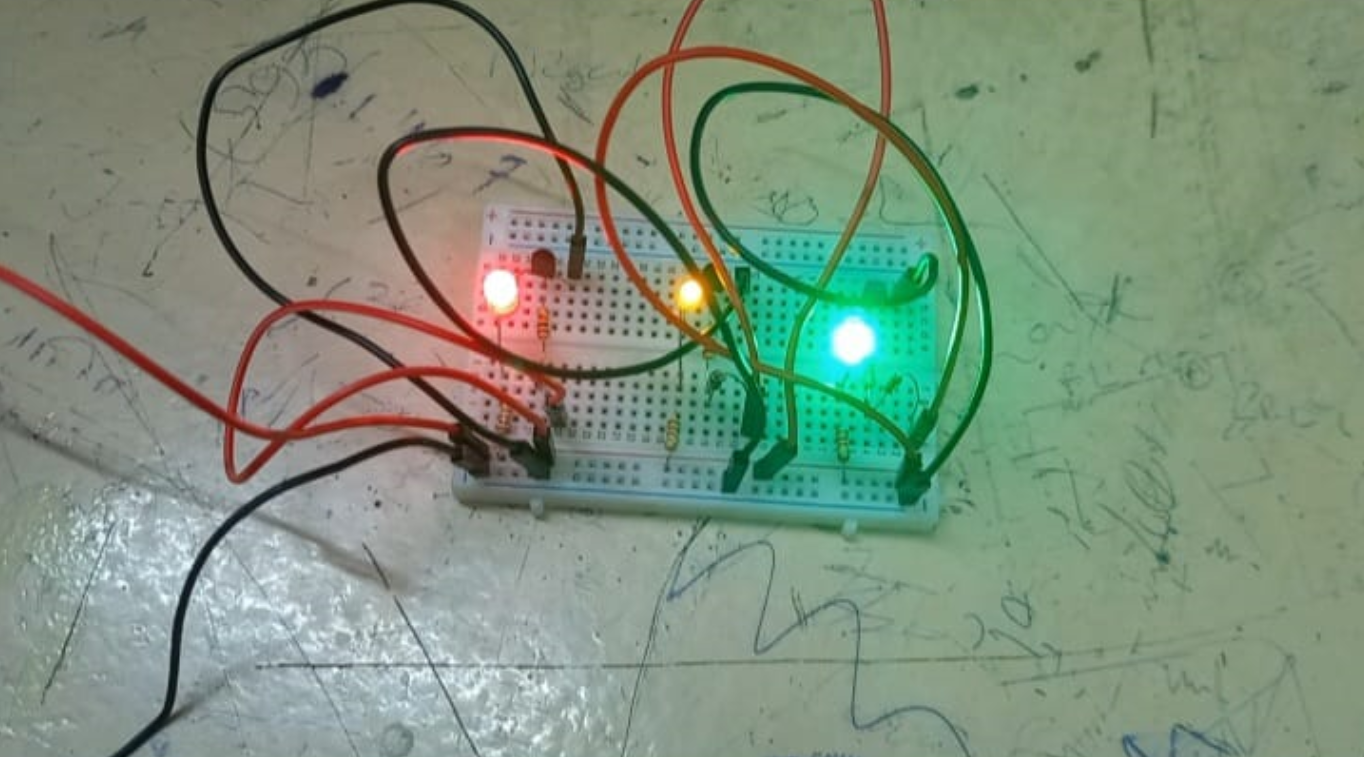
\includegraphics[width=0.5\textwidth]{12.png} % Replace 'diagram.png' with your image file
    \caption{Research Method}
    \label{fig:sample}
\end{figure}
